\chapter{Resultados}
\label{ch:resultados}

La propia estructuración de los objetivos definidos para este trabajo de fin de grado servirá como base para la exposición de los resultados. De esta manera, se obtendrá un enfoque global, y a la vez, detallado, de cada una de las partes que componen el proyecto.

Para ello, al igual que en puntos anteriores, esta sección se dividirá en tres partes bien diferenciadas: Desarrollo del circuito electrónico, diseño de algoritmos y programación y tareas orientadas a la seguridad del dispositivo.
\section{Construcción del circuito electrónico}

La construcción del circuito electrónico definida en la fase de planificación contaba con dos objetivos principales, que eran los de realizar las conexiones necesarias para el correcto funcionamiento del dispositivo y fijar los elementos de manera segura y firme.

\begin{figure}[tbp]
\centering
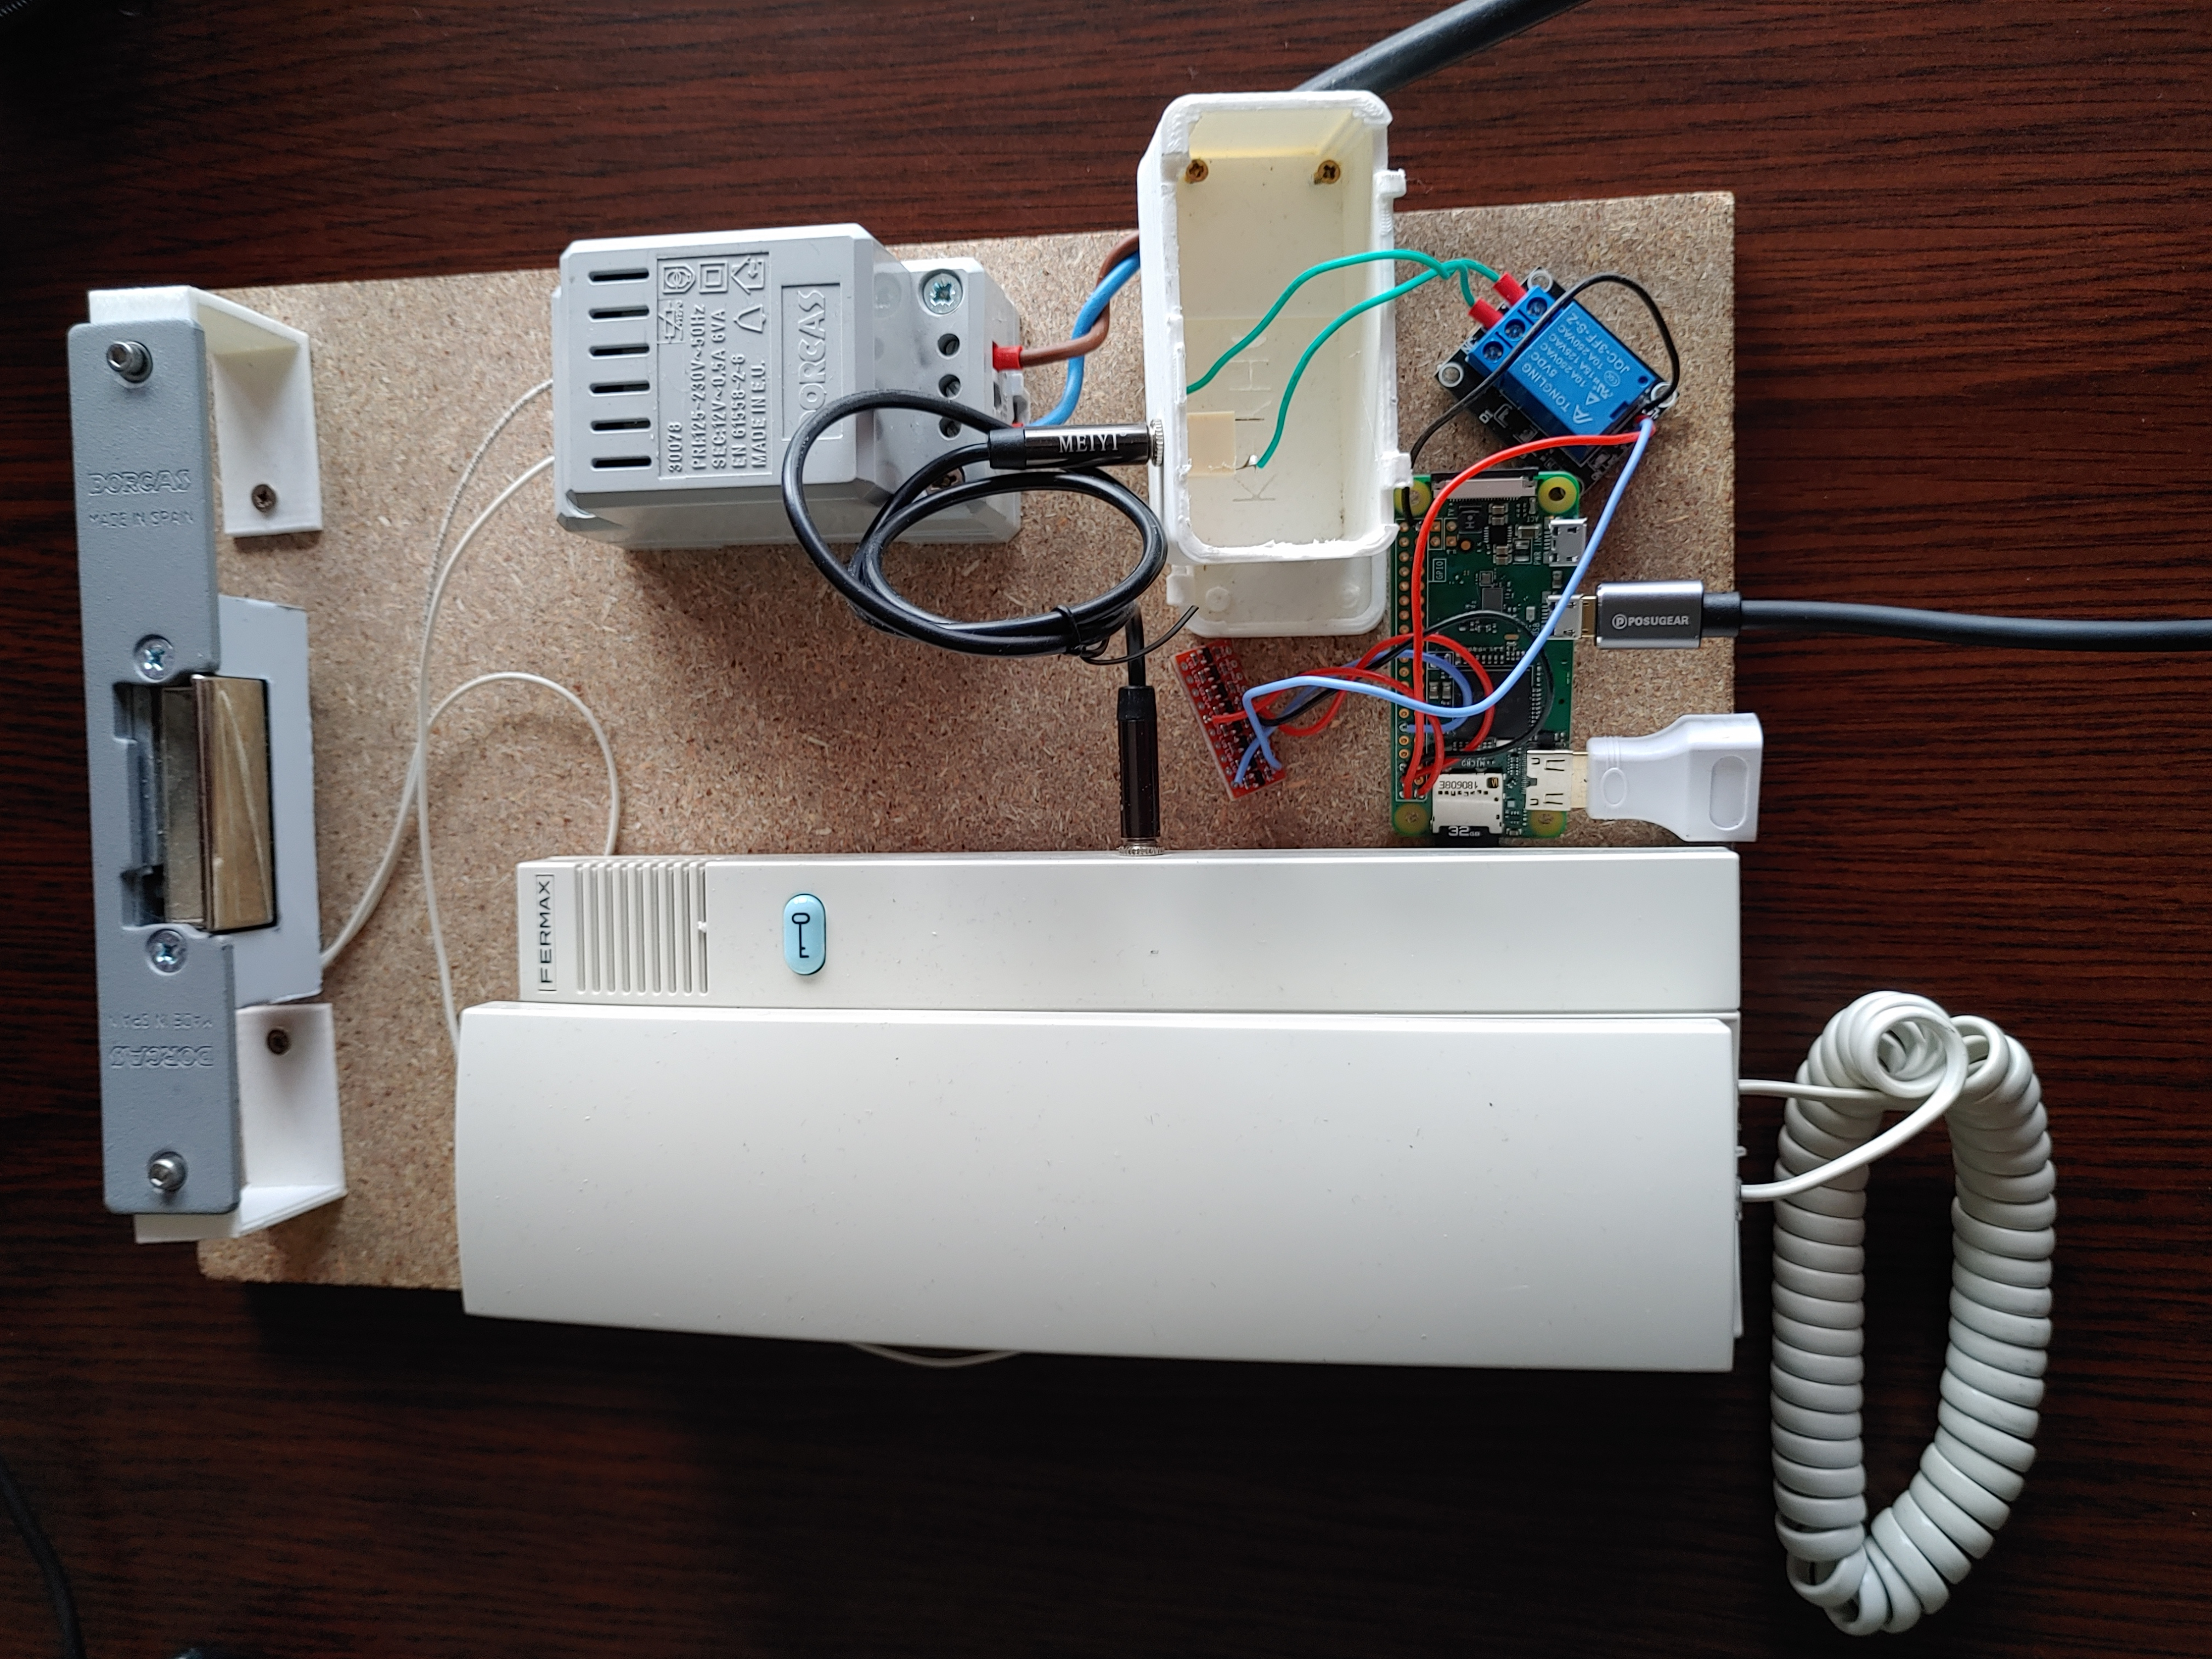
\includegraphics[scale = 0.1]{Prototipo_Completo.jpg}
\caption{Prototipo completo con todas las conexiones}
\label{fig:prototipo-completo}
\end{figure}
\begin{figure}[tbp]
\centering
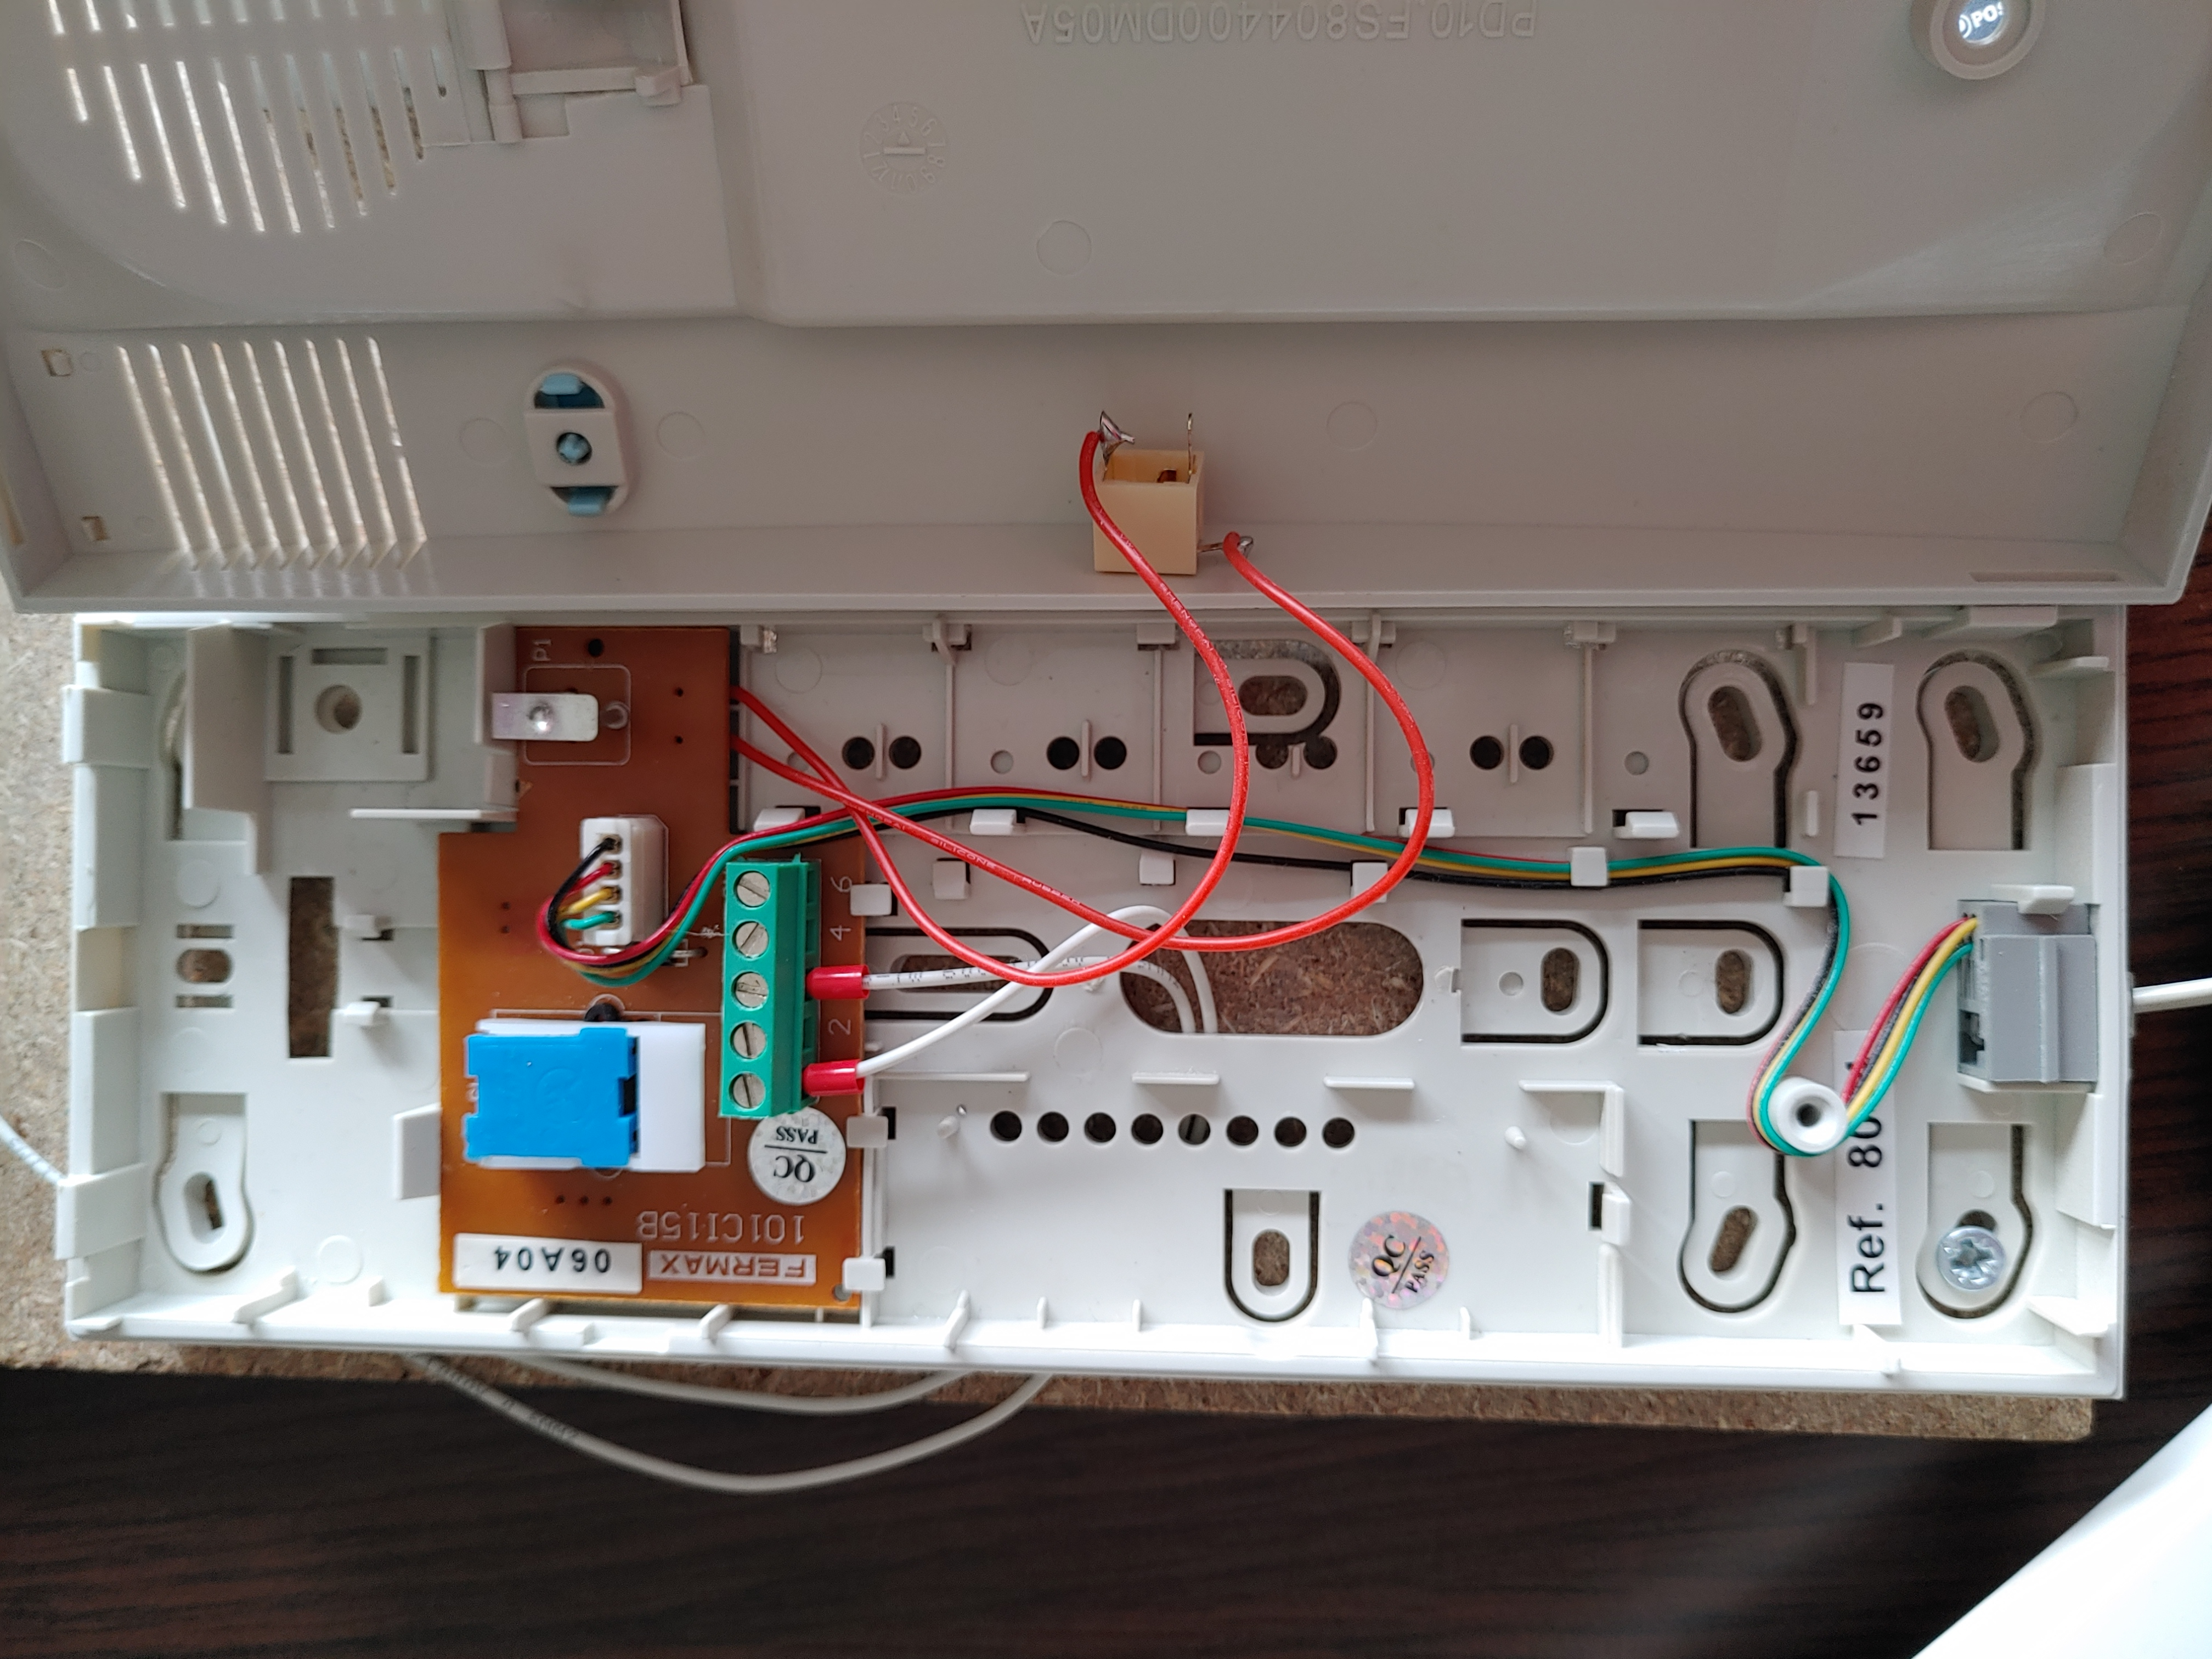
\includegraphics[scale = 0.1]{Interior_Portero_Automatico.jpg}
\caption{Conexiones en el interior del portero automático}
\label{fig:interior-portero-automatico}
\end{figure}

En las figura~\ref{fig:prototipo-completo} y ~\ref{fig:interior-portero-automatico} se puede observar el prototipo con todos los elementos que lo forman interconectados entre sí, tal como se definió en la fase de desarrollo. Tanto el portero automático, como la cerradura eléctrica y el transformador, han sido fijados por medio de tornillería a un tablón de madera que permite realizar, de forma segura y compacta, el transporte del prototipo.

Junto a estos elementos, puede observarse la interconexión de la Raspberry Pi Zero W con el conversor de nivel lógicos y el relé, que permiten el correcto funcionamiento de este prototipo.

La interconexión que adapta el sistema con el portero automático se ha hecho por medio de un conector tipo mini jack, con la intención de hacer que sea más intuitivo para el usuario final.

Queda expuesto por tanto, de forma gráfica, como los dos puntos principales que quedaron definidos para esta fase inicial han sido cumplidos de forma exitosa.

\section{Diseño de algoritmos y programación}
En el apartado de planificación del presente trabajo queda constancia de las diferentes materias que debían tenerse en cuenta en lo referente al diseño de algoritmos y programación.

\subsection{Programa capaz de activar la cerradura en los momentos precisos}

La primera característica que se implementa en el proyecto es la de hacer un programa capaz de activar una señal que permita realizar la apertura de la cerradura, ayudándose para ello del circuito construido previamente. Este programa debía poder estar controlado por un administrador que contara con la posibilidad de crear y anular reservas, realizar la apertura de la puerta y dejar las tareas de administración.

Una vez realizada la integración de los códigos implementados en la fase de desarrollo, y ejecutados por medio de la Raspberry Pi, se obtienen los resultados esperados, dando lugar a un panel de administración como el que se observa en la figura~\ref{fig:panel-de-administrador}.
\begin{figure}[tbp]
\centering
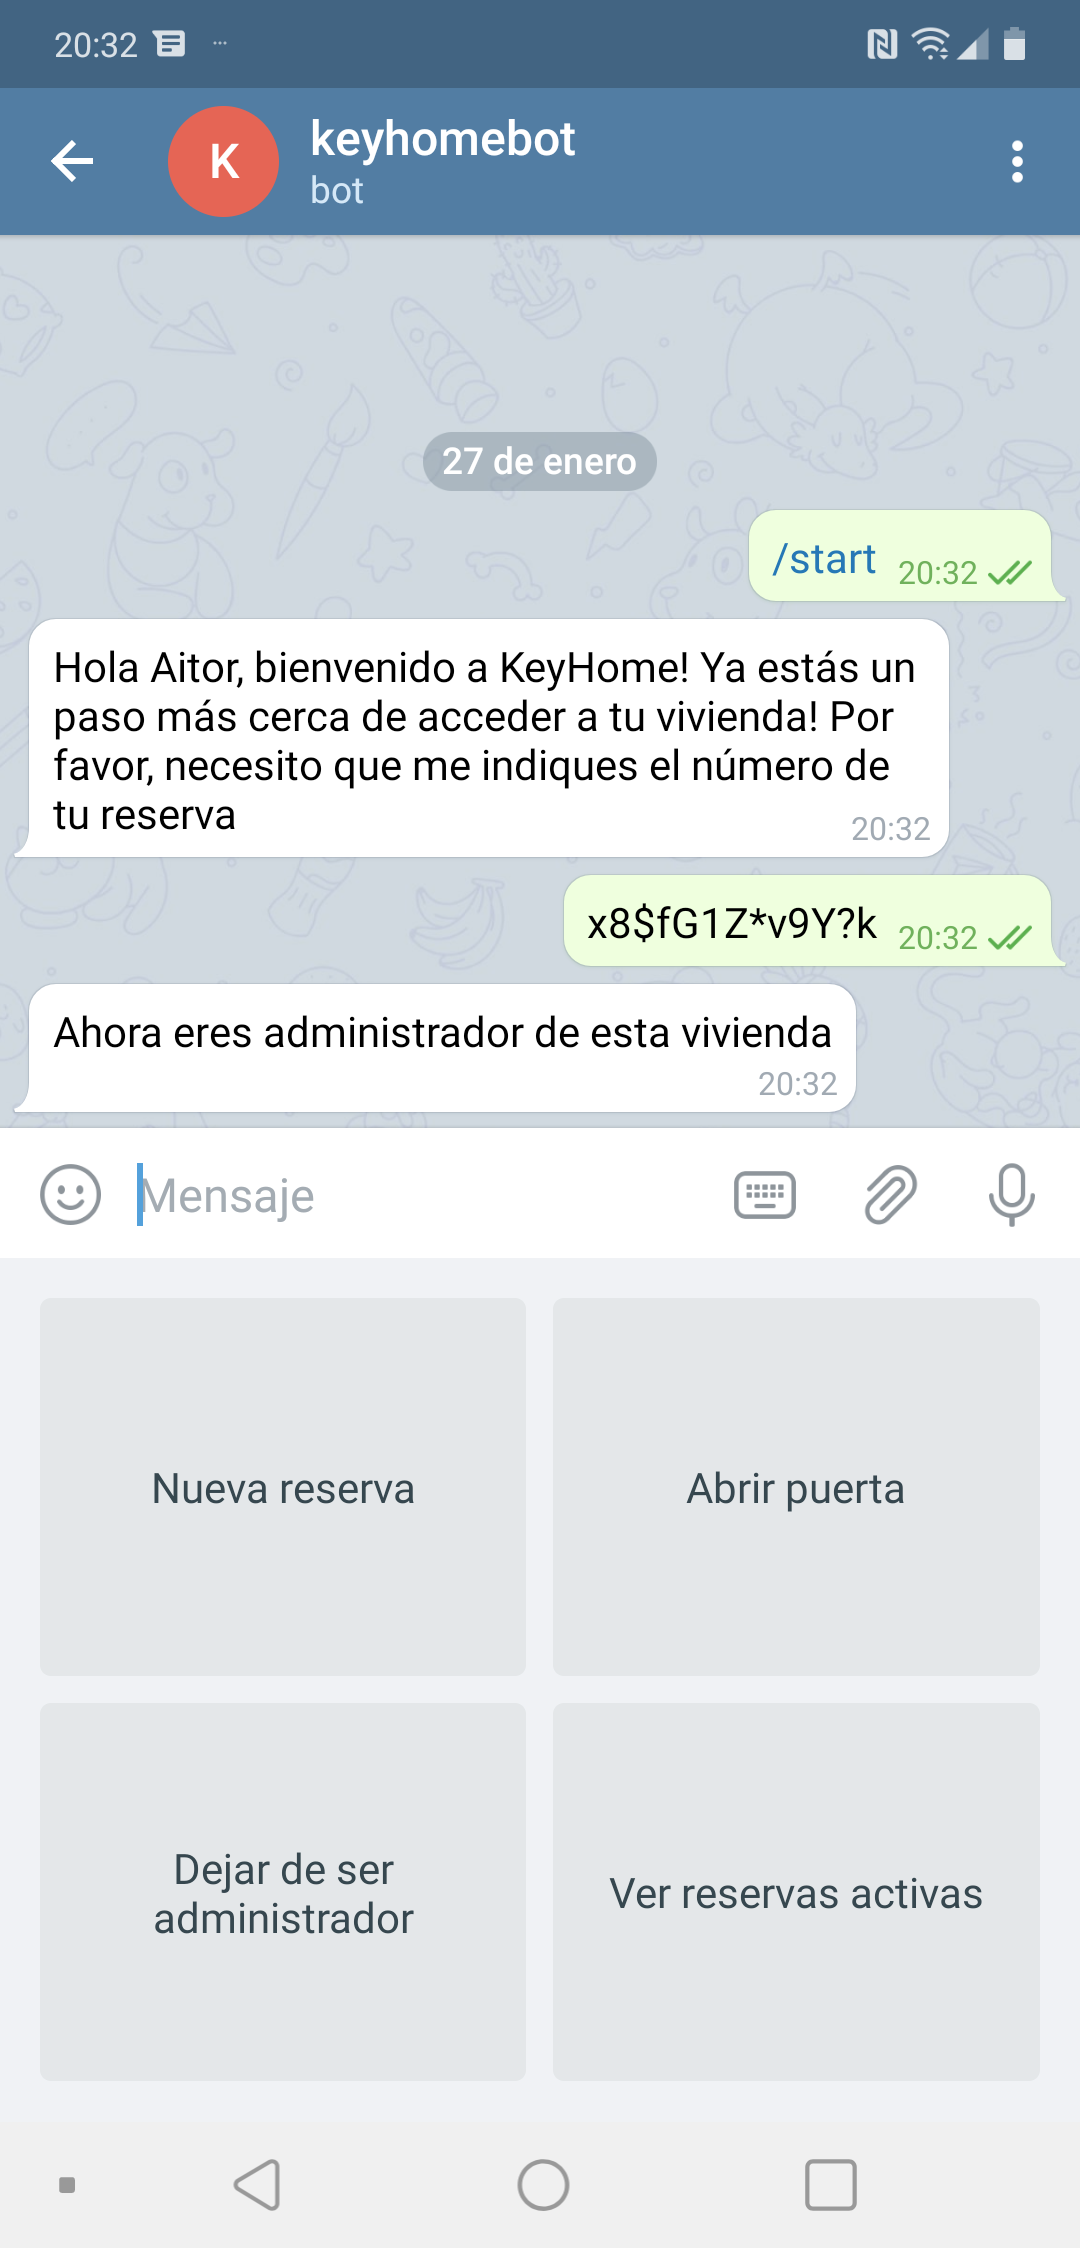
\includegraphics[scale = 0.15]{fig/Panel_de_administrador.png}
\caption{Panel de administrador}
\label{fig:panel-de-administrador}
\end{figure}

\subsubsection{Creación de nuevas reservas}

Entre las tareas de este apartado, destacan aquellas que tienen por objeto automatizar la entrada de nuevas reservas en el sistema. Sin embargo, por diferentes razones, es recomendable incluir la posibilidad al administrador de que él mismo pueda añadir estas reservas. Para ello, en la figura~\ref{fig:panel-de-administrador} se puede observar como se ha creado un apartado de crear reservas. Si hacemos uso de esta opción, el bot pedirá, en primer lugar, que se indique el número de reserva, tal como se puede observar en la figura~\ref{fig:introduccion-del-numero-de-reserva}. Este número de reserva será aquel con el que el huésped podrá acceder a la vivienda el día en que comience su estancia.
\begin{figure}[tbp]
\centering
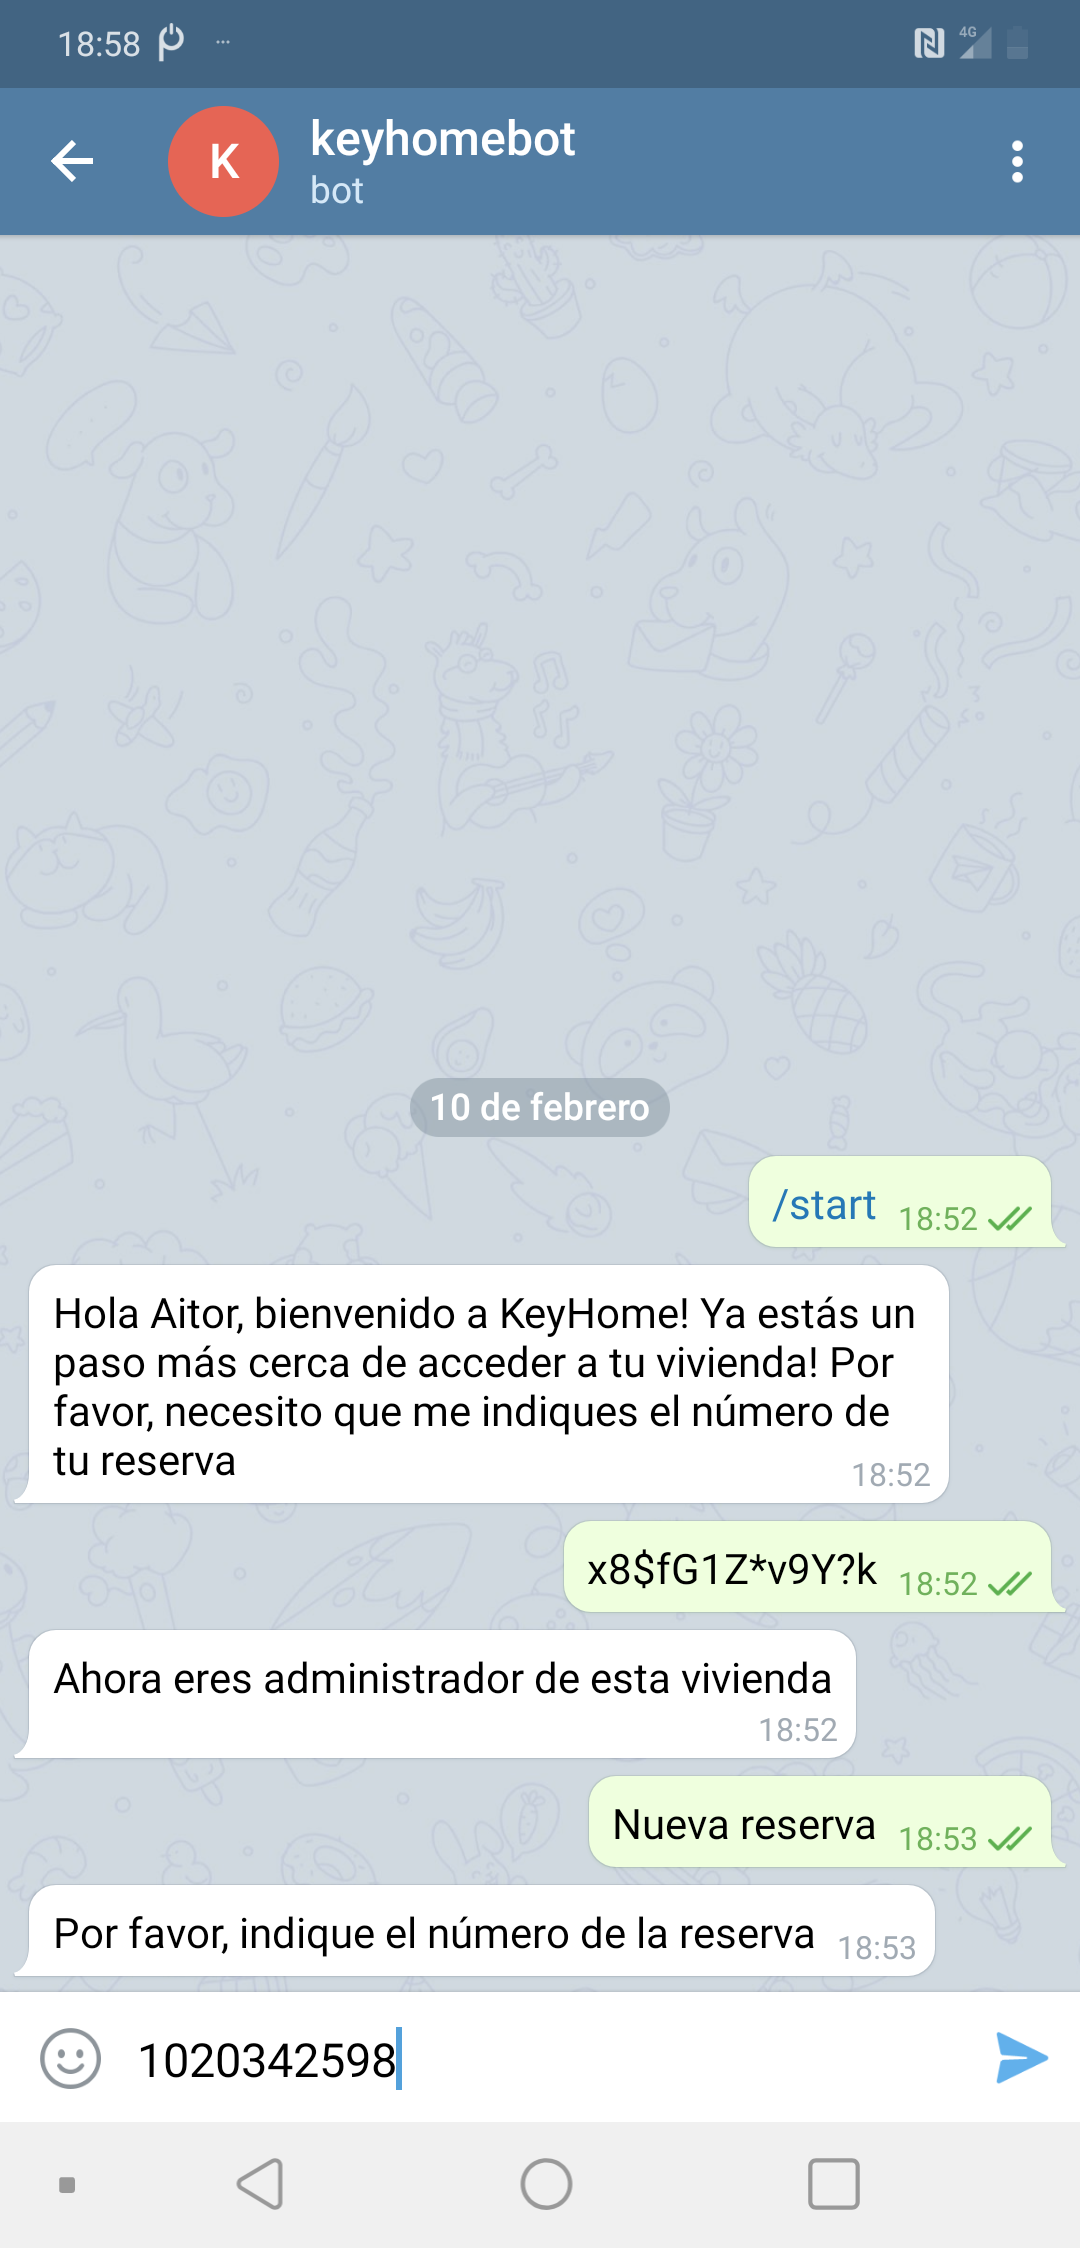
\includegraphics[scale = 0.15]{fig/Numero-de-reserva.png}
\caption{Introducción del número de reserva}
\label{fig:introduccion-del-numero-de-reserva}
\end{figure}

Una vez que el administrador introduzca el número de reserva, lo siguiente que le es exigido por parte del bot son las fechas de entrada y de salida del cliente, tal como puede observarse en la figura~\ref{fig:introduccion-de-las-fechas-de-reserva}, donde se establecen las fechas en las que el cliente podrá acceder a la vivienda.

\begin{figure}[tbp]
\centering
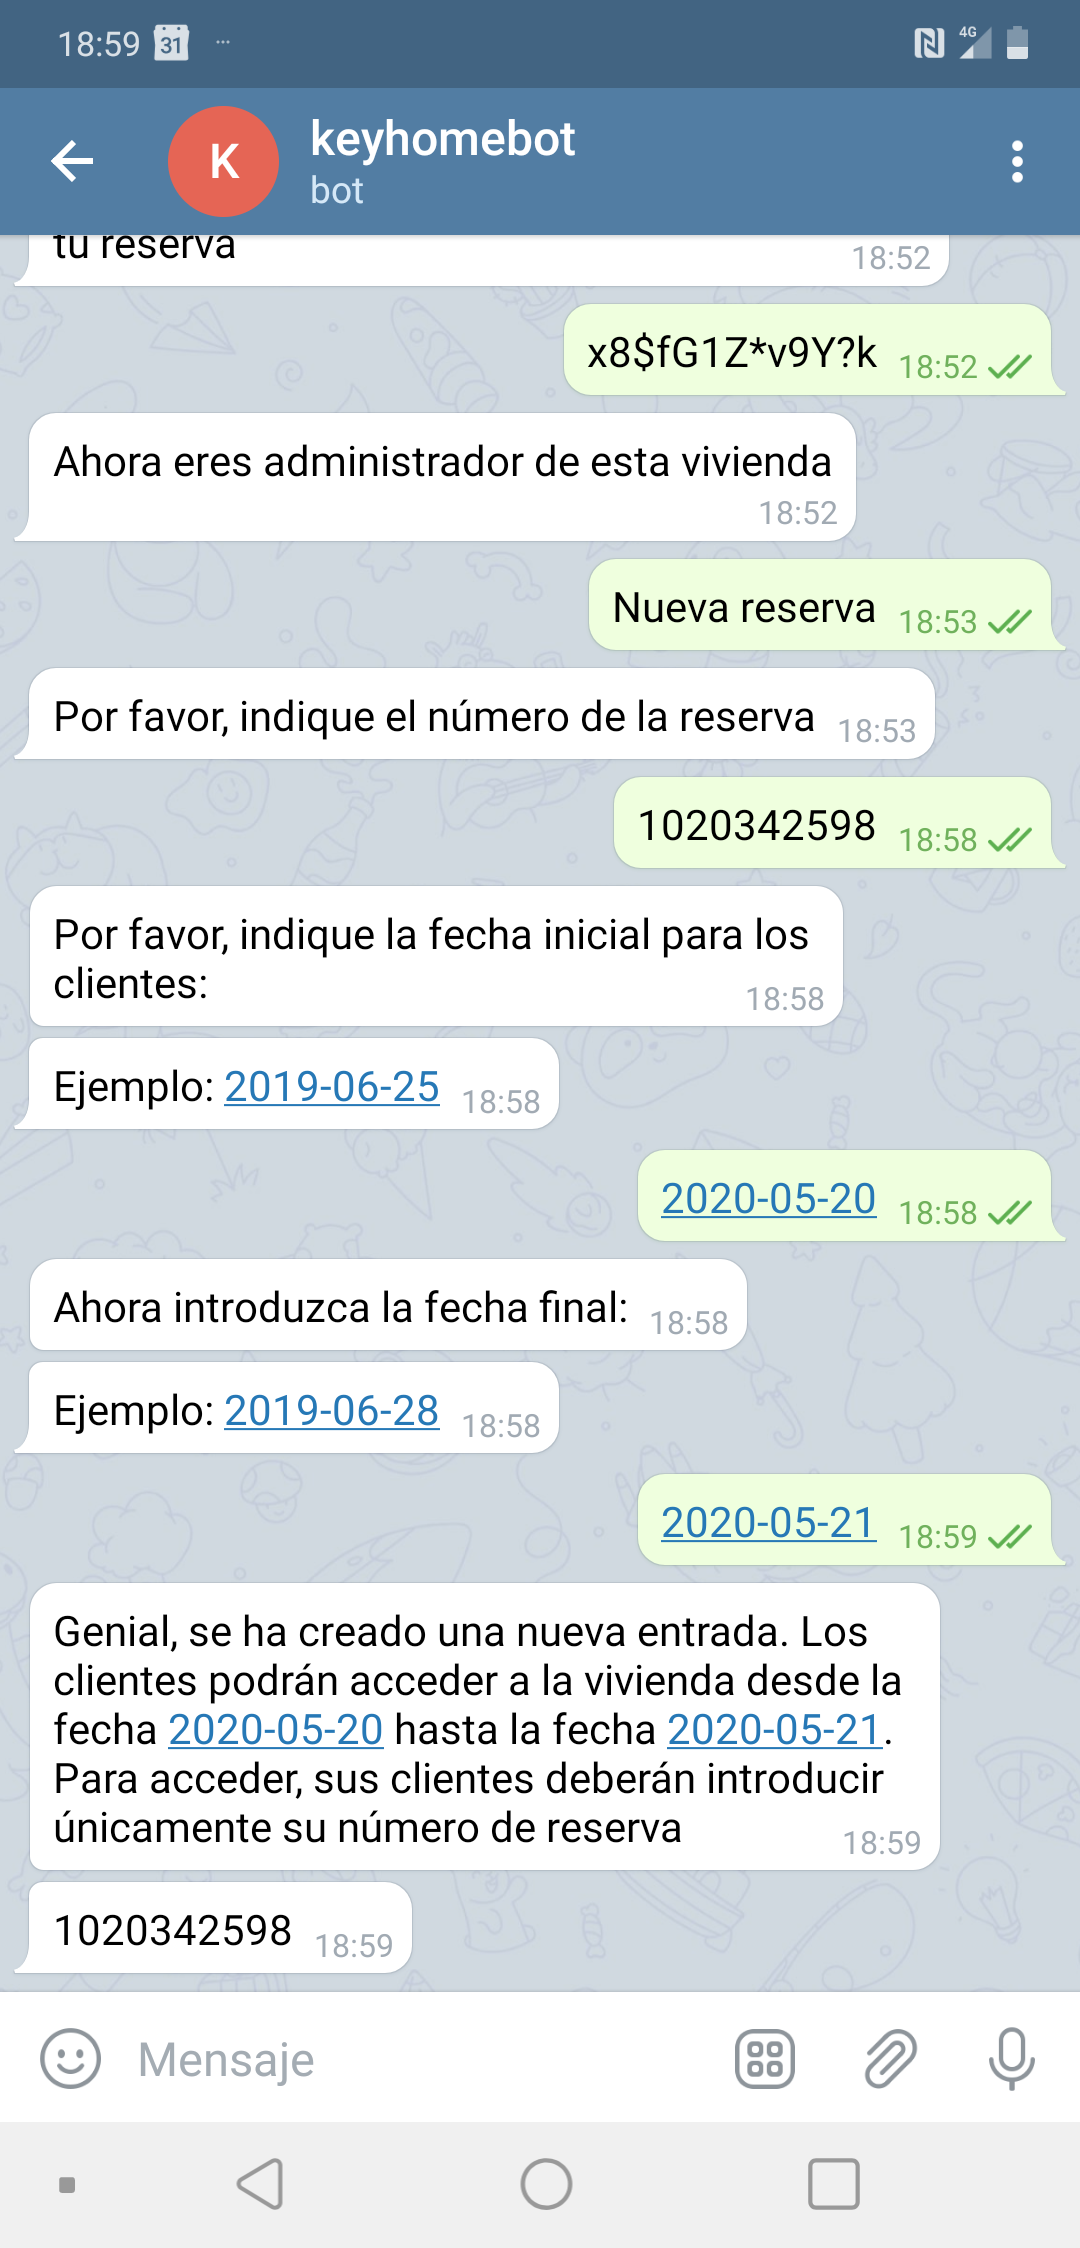
\includegraphics[scale = 0.15]{fig/Fechas-de-reserva.png}
\caption{Introducción de las fechas de reserva}
\label{fig:introduccion-de-las-fechas-de-reserva}
\end{figure}

\subsubsection{Apertura de la cerradura por parte del administrador}

La siguiente función que debe cumplirse, siguiendo la programación de las tareas, sería la de permitir que el administrador de la vivienda tuviese la posibilidad de abrir la puerta. Esta posibilidad queda habilitada en el programa central definido en el apartado de desarrollo de este documento, a través del cual se crea el resultado que se muestra en la figura~\ref{fig:apertura-de-puerta-por-parte-del-administrador}, donde un administrador activa la apertura de la cerradura desde su panel de control.

\begin{figure}[tbp]
\centering
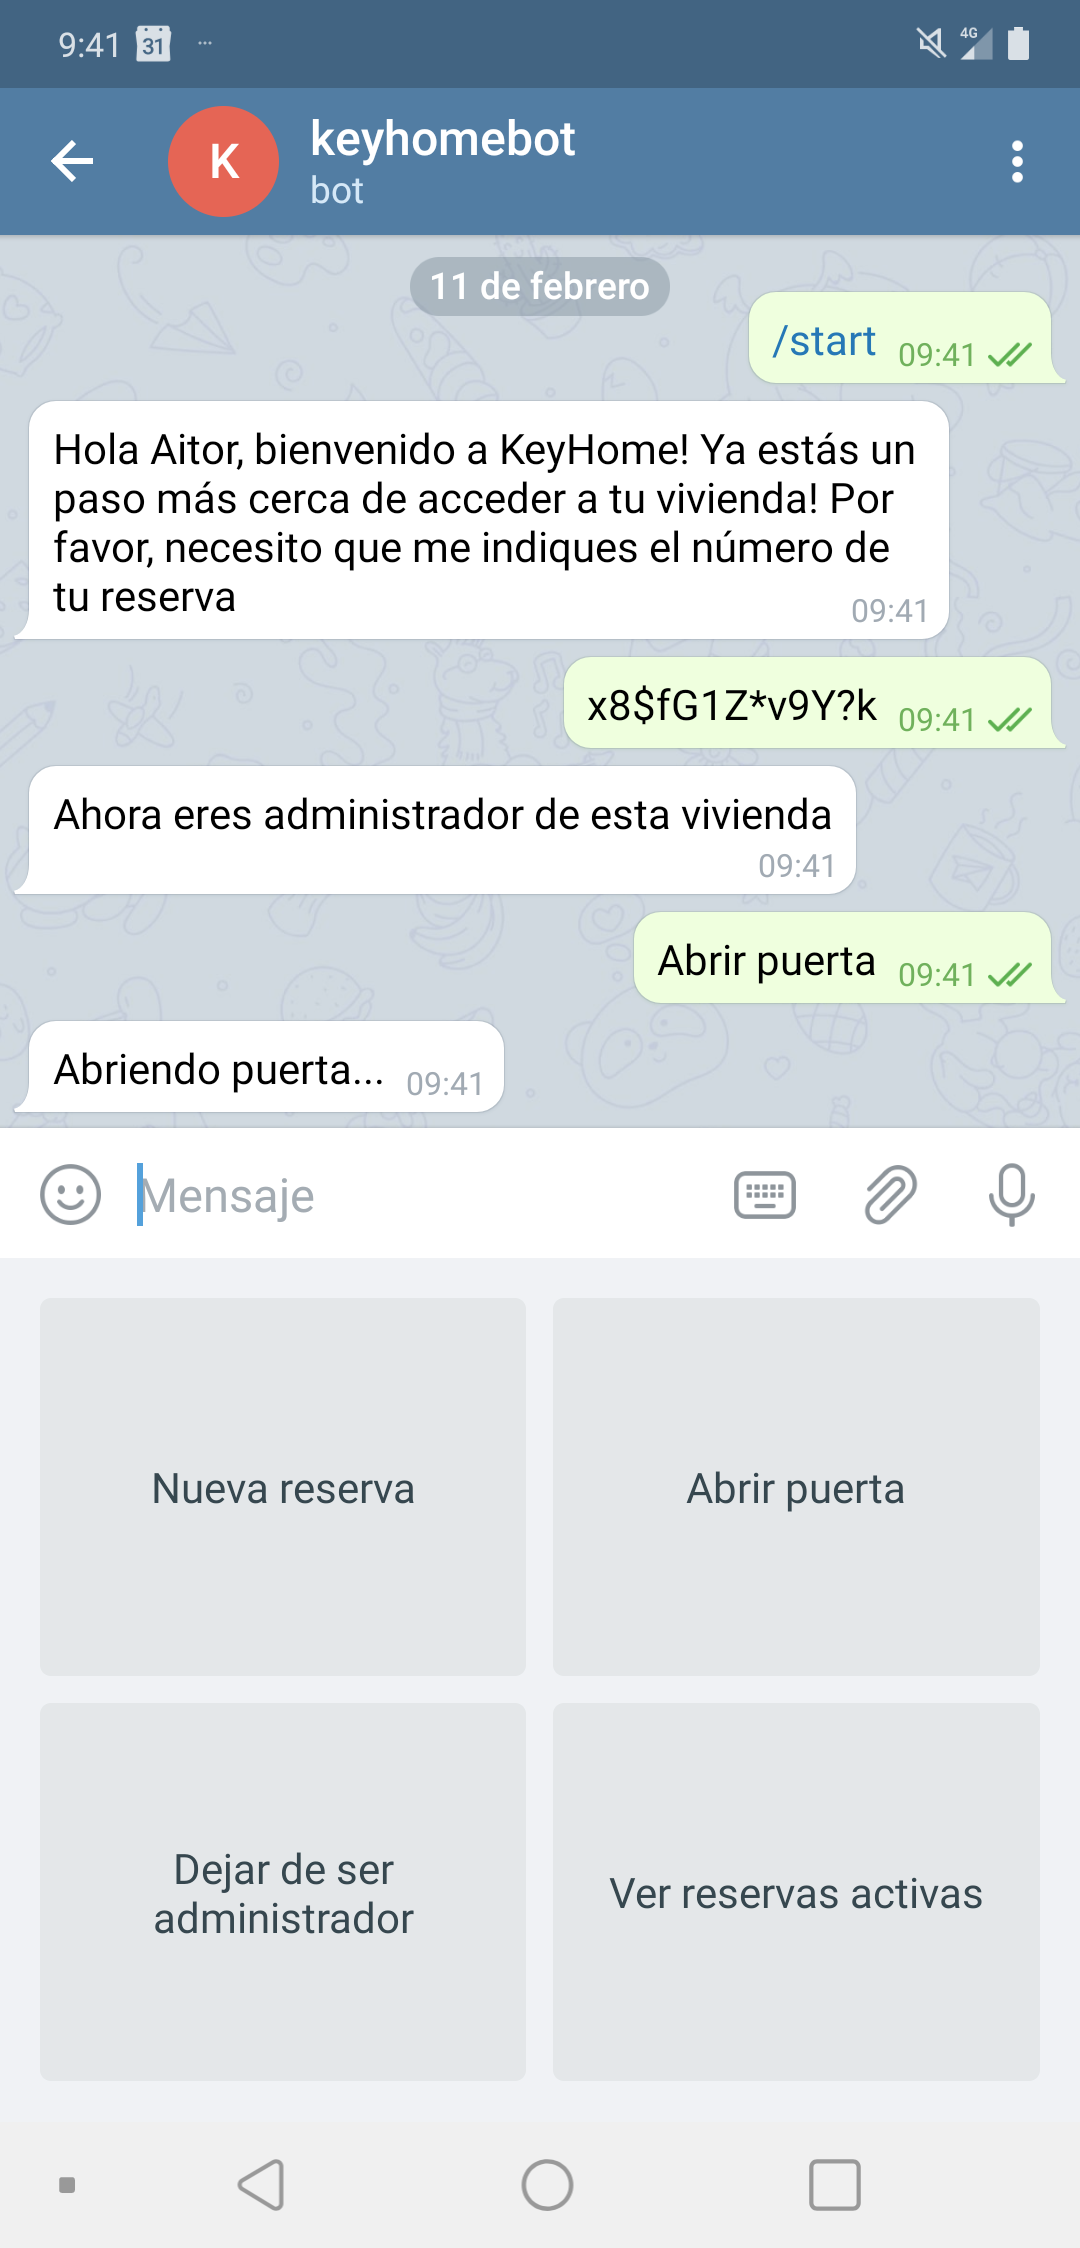
\includegraphics[scale=0.15]{fig/Apertura-de-puerta-administrador.png}
\caption{Apertura de puerta por parte del administrador}
\label{fig:apertura-de-puerta-por-parte-del-administrador}
\end{figure}

\subsubsection{Dejar permisos de administrador}

Por diferentes razones, se puede dar la situación de que una persona que ha sido administradora de la vivienda durante un tiempo, no deba continuar ejerciendo como tal. Para ello, se decidió habilitar esta aplicación con la posibilidad de dejar ese cargo, tal como puede observarse en la figura~\ref{fig:administrador-dejando-sus-permisos-de-administracion}, donde un administrador deja los permisos como administrador.

\begin{figure}[tbp]
\centering
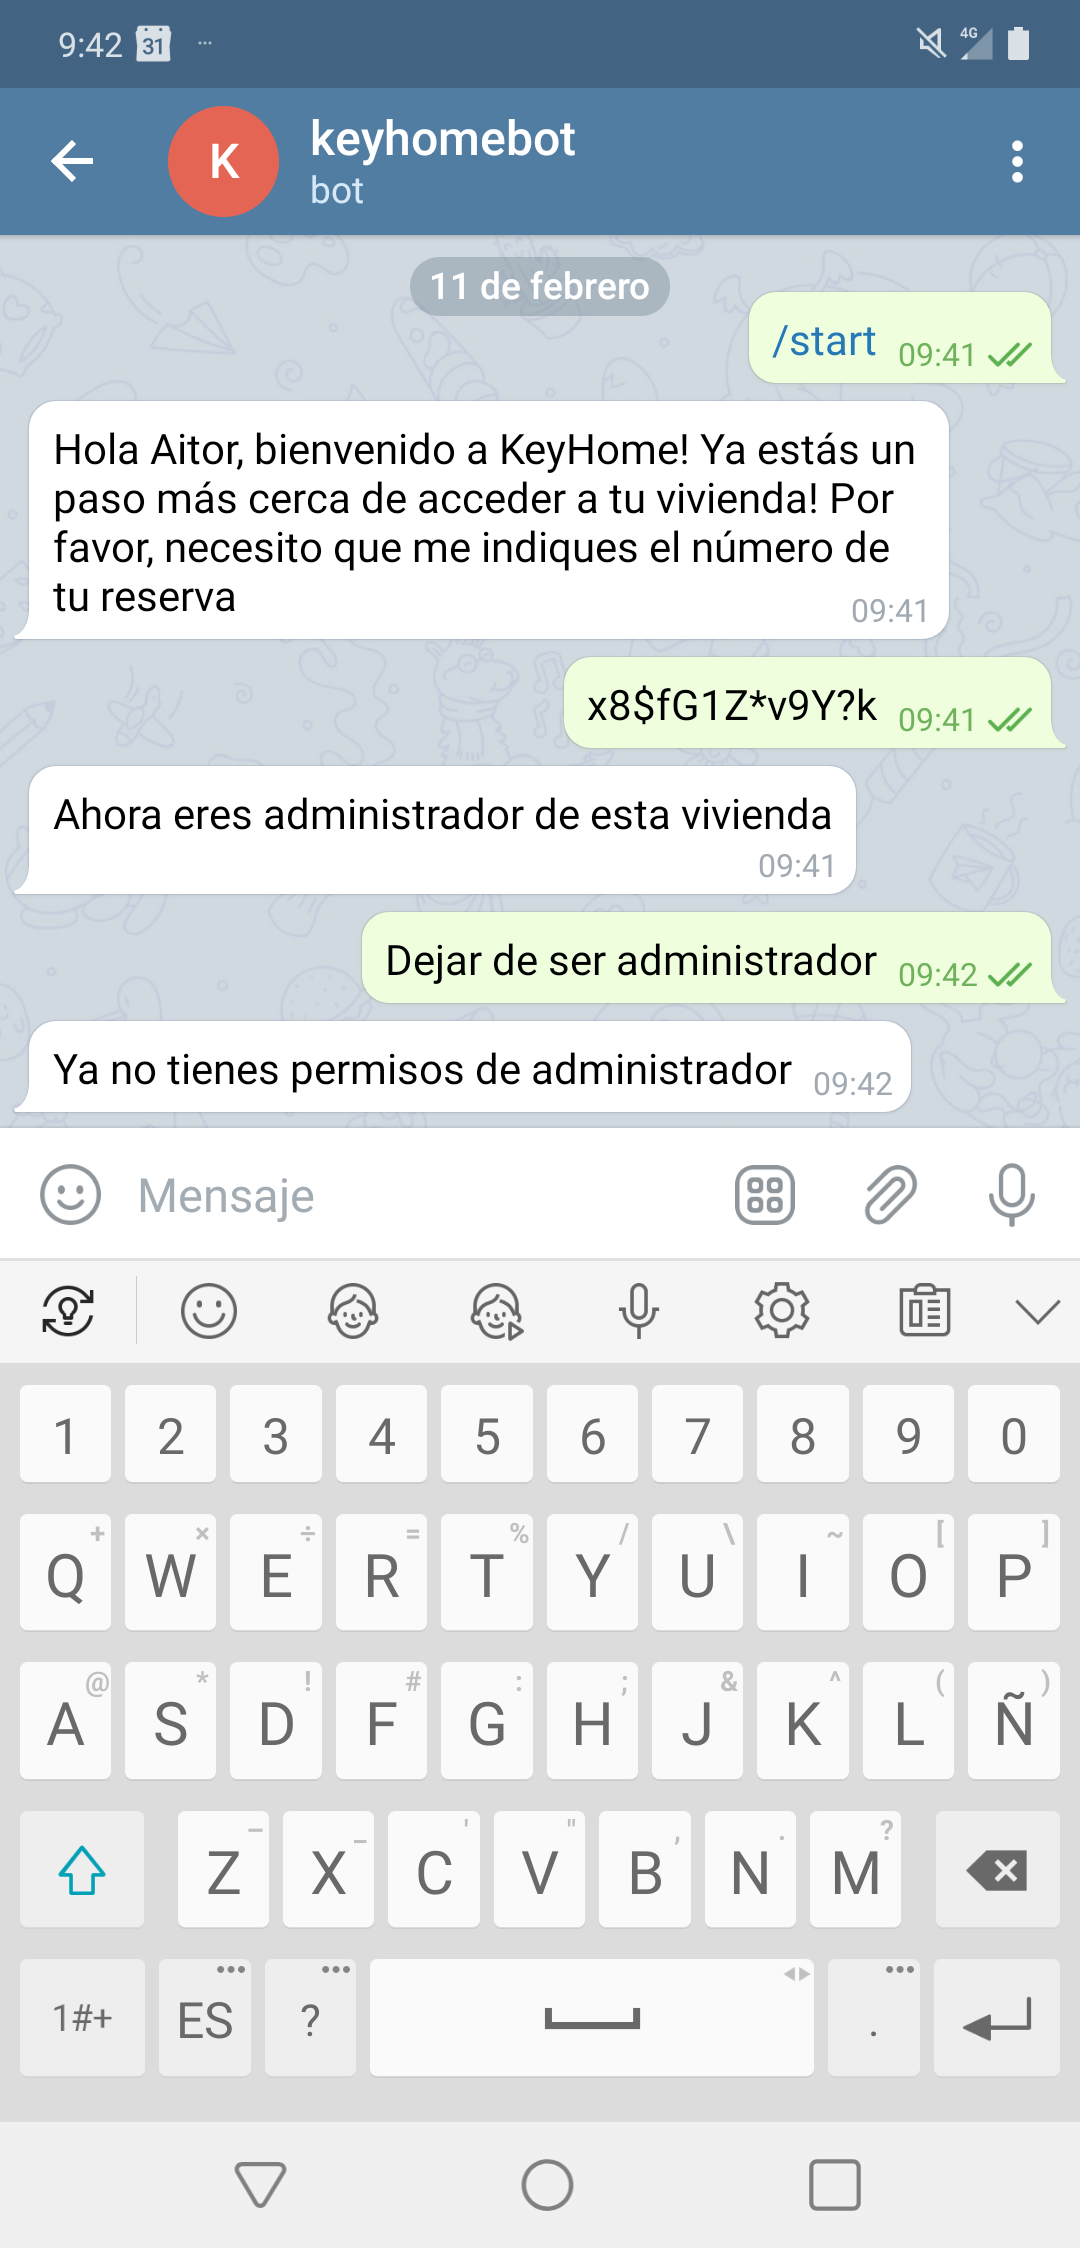
\includegraphics[scale=0.15]{fig/Dejar-de-ser-administrador.png}
\caption{Administrador dejando sus permisos de administración}
\label{fig:administrador-dejando-sus-permisos-de-administracion}
\end{figure}

\subsubsection{Consulta y modificación de reservas}

El último punto que se determinó añadir a los poderes de administrador, fue el de incluir la posibilidad de consultar las reservas, y además, poder anular aquellas que se considere. Es en la figura~\ref{fig:consulta-y-moficicacion-de-reservas}, donde se observa como el administrador de la vivienda consulta las diferentes fechas que hay disponibles, eliminando una de ellas a modo de ejemplo.

\begin{figure}[tbp]
\centering
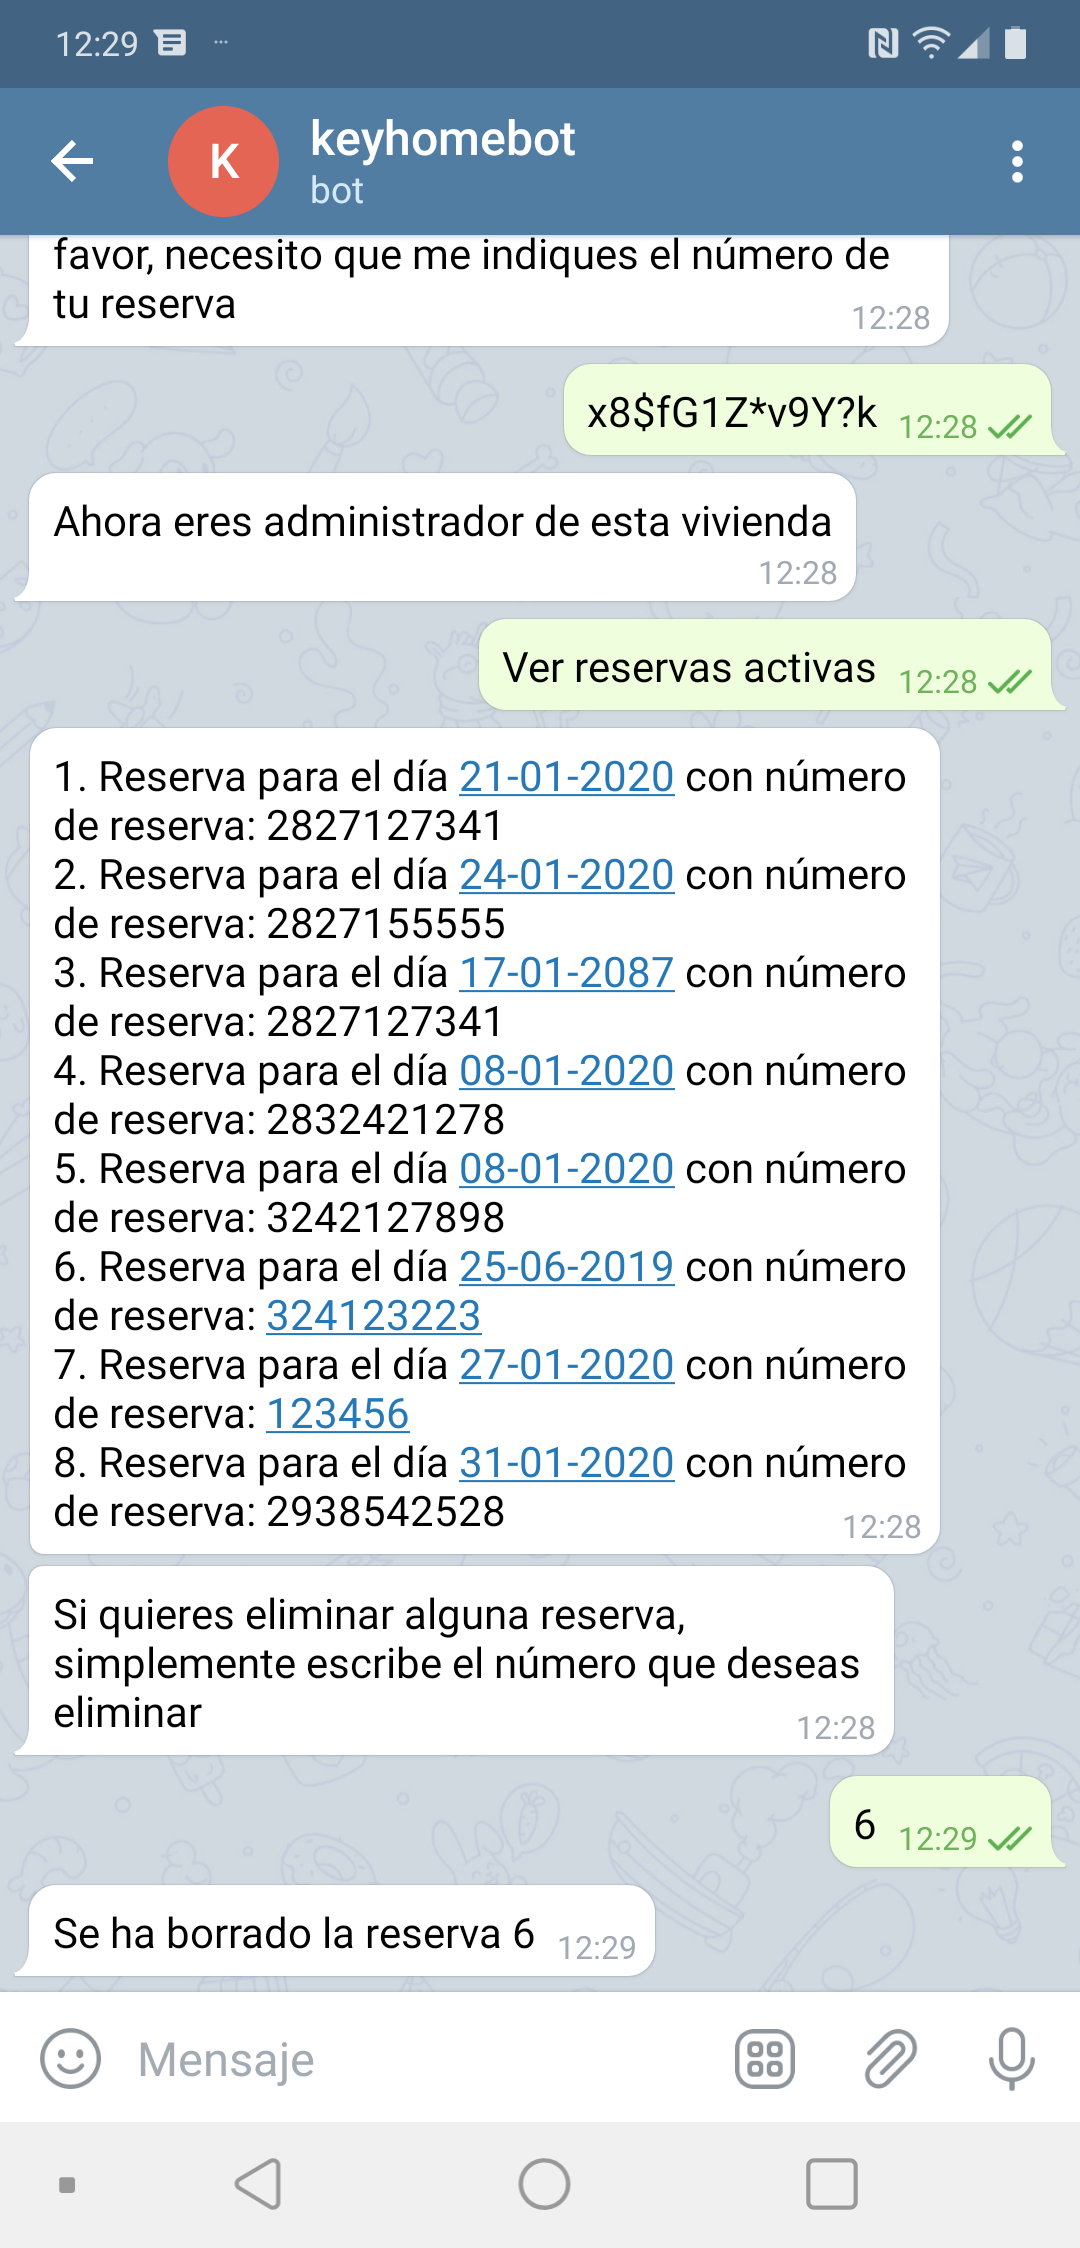
\includegraphics[scale=0.15]{fig/Consulta-y-modificacion-reservas.png}
\caption{Consulta y modificación de reservas}
\label{fig:consulta-y-moficicacion-de-reservas}
\end{figure}

A parte del administrador, la única figura que forma parte de este proyecto es la del usuario final o huésped de la vivienda, el cual debe tener a su disposición la posibilidad de abrir la puerta en el momento de su llegada. En la figura~\ref{fig:apertura-de-puerta-por-parte-del-huesped} puede observarse como este usuario final introduce su número de reserva, y al estar activo en ese momento, se le permite acceder a la vivienda realizando la apertura automática de la cerradura.

\begin{figure}[tbp]
\centering
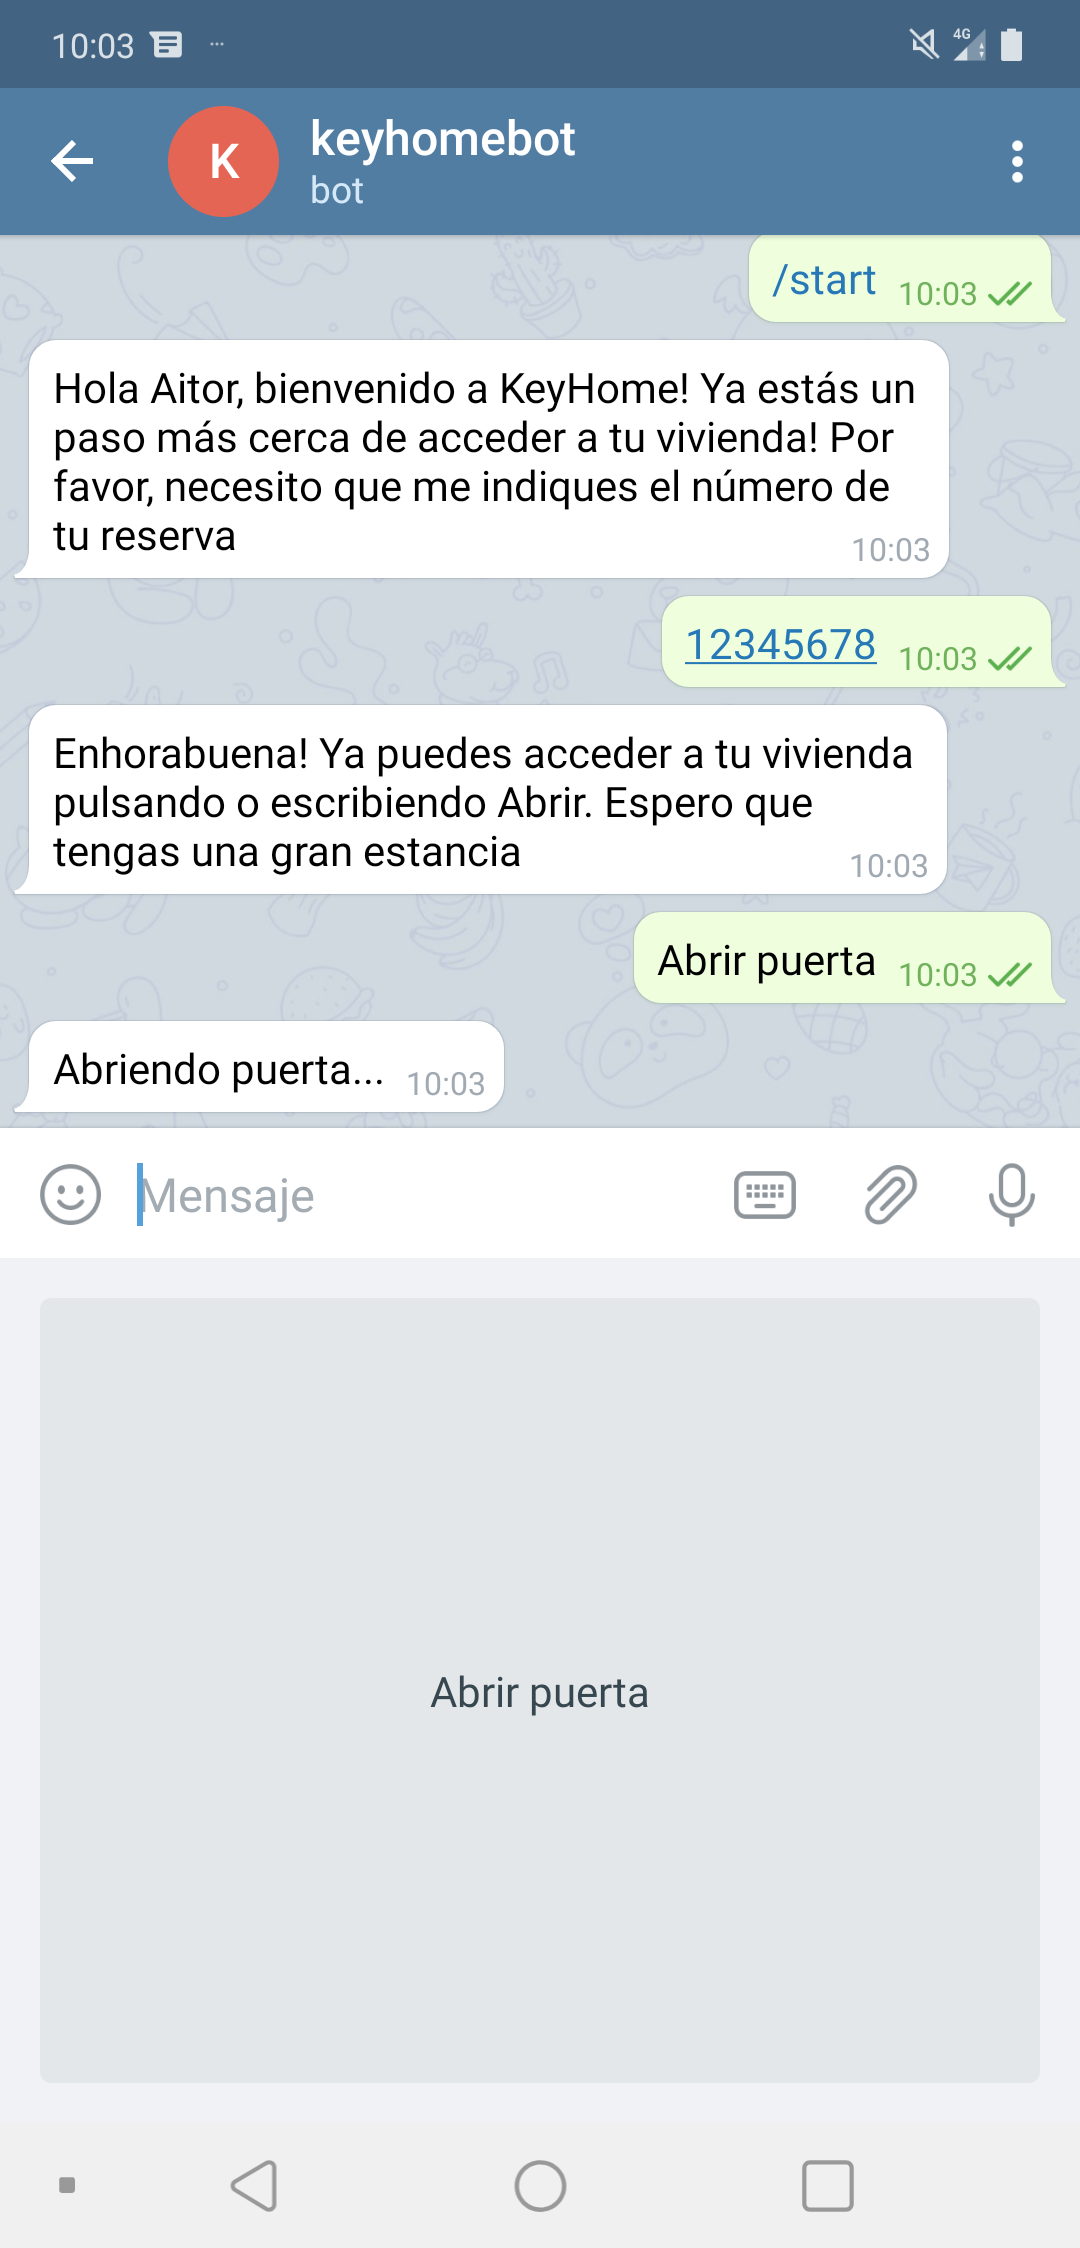
\includegraphics[scale=0.15]{fig/Apertura-de-puerta-por-parte-del-huesped.png}
\caption{Apertura de la cerradura por parte del huésped}
\label{fig:apertura-de-puerta-por-parte-del-huesped}
\end{figure}

\subsubsection{Automatización de la entrada y cancelación de reservas}

Existen muchas plataformas de alquiler vacacional. Para la elaboración de este sistema automático de recepción de reservas se ha hecho un programa, descrito en el apartado de desarrollo del presente documento, que automatiza las reservas de la plataforma Booking. Se ha tomado esta decisión, en base a dos razones principales:
\begin{enumerate}
\item Es la plataforma más utilizada en la actualidad.
\item Para la elaboración de este programa se ha podido utilizar el modelo de correo que envía Booking en la actualidad, con lo que la automatización descrita en este punto es completamente funcional.
\end{enumerate}

El resultado obtenido en este apartado ha sido el esperado, ya que ante una entrada de nueva reserva, notificada a la aplicación por medio de correo electrónico recibido de Booking, se ha conseguido incorporar dicha reserva en el historial de reservas que pueden ser consultados y modificados por el anfitrión. De igual manera, cuando Booking informa de una cancelación, por medio de un correo electrónico, este es recibido por el programa descrito en el apartado de desarrollo, el cual se encarga de eliminar dicha reserva del sistema incorporado en la Raspberry Pi, eliminando así toda posibilidad de acceso para el cliente que ha cancelado.

\subsection{Seguridad del dispositivo}
Al igual que en los puntos que preceden a este, la metodología de análisis de resultados consistirá en evaluar los frutos que han sido obtenidos del trabajo desempeñado en la fase de desarrollo.

El primer programa que se realizó consistía en un sistema de detección que avisara al propietario en caso de que alguien abriera la caja donde se encuentra el circuito.
El funcionamiento de este programa es correcto, actuando de manera que, en caso de que alguien abra la caja, el detector de distancia ofrecerá una medida mayor, y ante tal suceso, el programa enviará un correo electrónico como el que puede verse en la figura~\ref{fig:aviso-ante-posible-manipulacion}.

\begin{figure}[tbp]
\centering
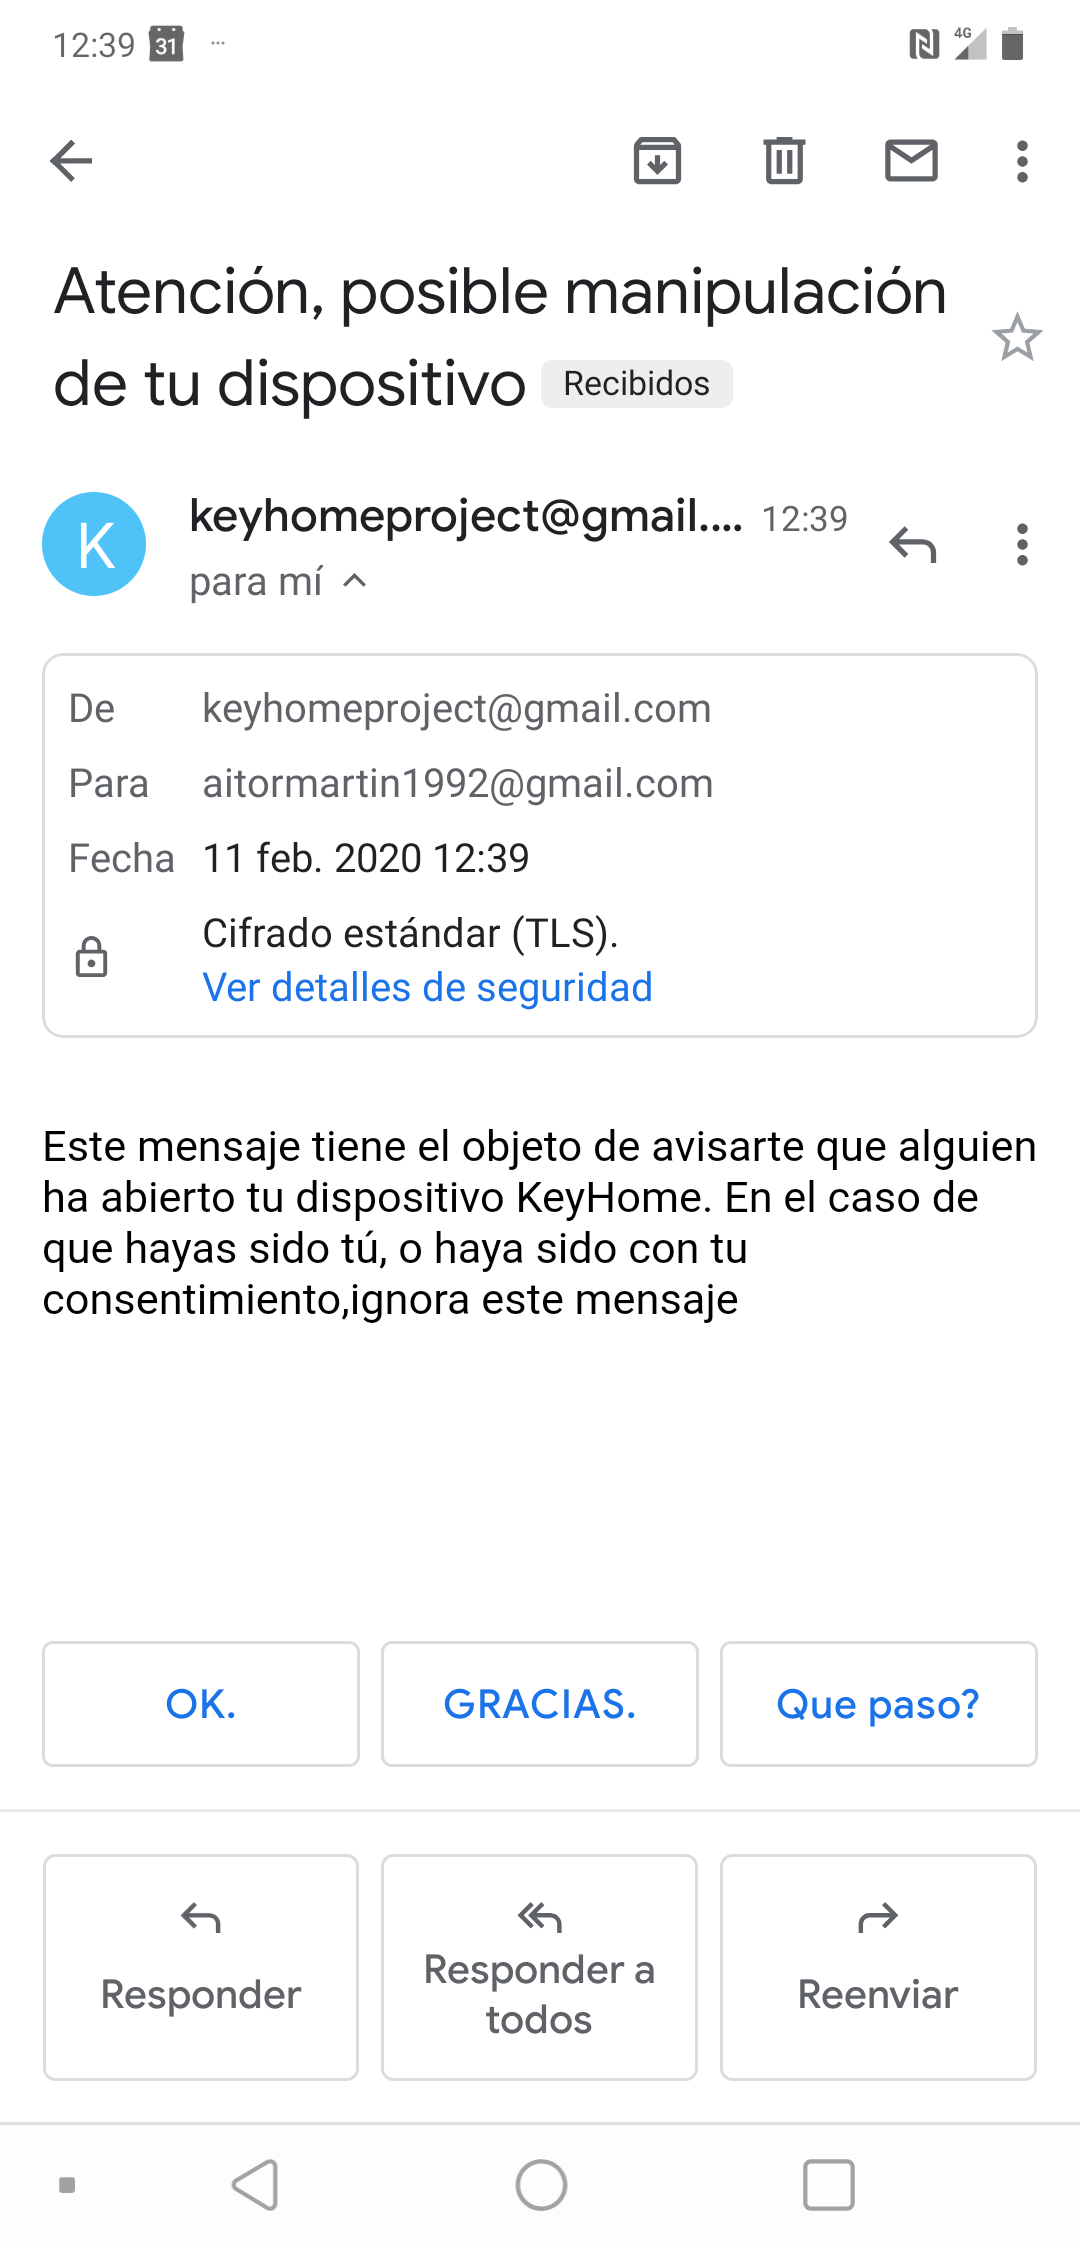
\includegraphics[scale=0.15]{fig/Aviso-ante-posible-manipulacion.png}
\caption{Aviso ante posible manipulación del dispositivo}
\label{fig:aviso-ante-posible-manipulacion}
\end{figure}

La desconexión, tanto a nivel eléctrico como de internet, del dispositivo, podría provocar múltiples situaciones negativas, como una posible manipulación o un cliente que no pudiera acceder a su vivienda. Para corregir esta situación, en la fase de desarrollo se decidió incluir un apartado en el que se avisara al propietario de forma remota. Para ello, se ha hecho uso de una plataforma llamada InitialState, que, tras la inclusión de ciertos scripts en la Raspberry Pi, recibe de forma continua señales de la ejecución del programa o programas que se deseen analizar. En la figura~\ref{fig:monitorizacion} puede observarse como, desde el ordenador, puede observarse de forma gráfica la frecuencia de trabajo de un programa en la Raspberry Pi.

\begin{figure}[tbp]
\centering
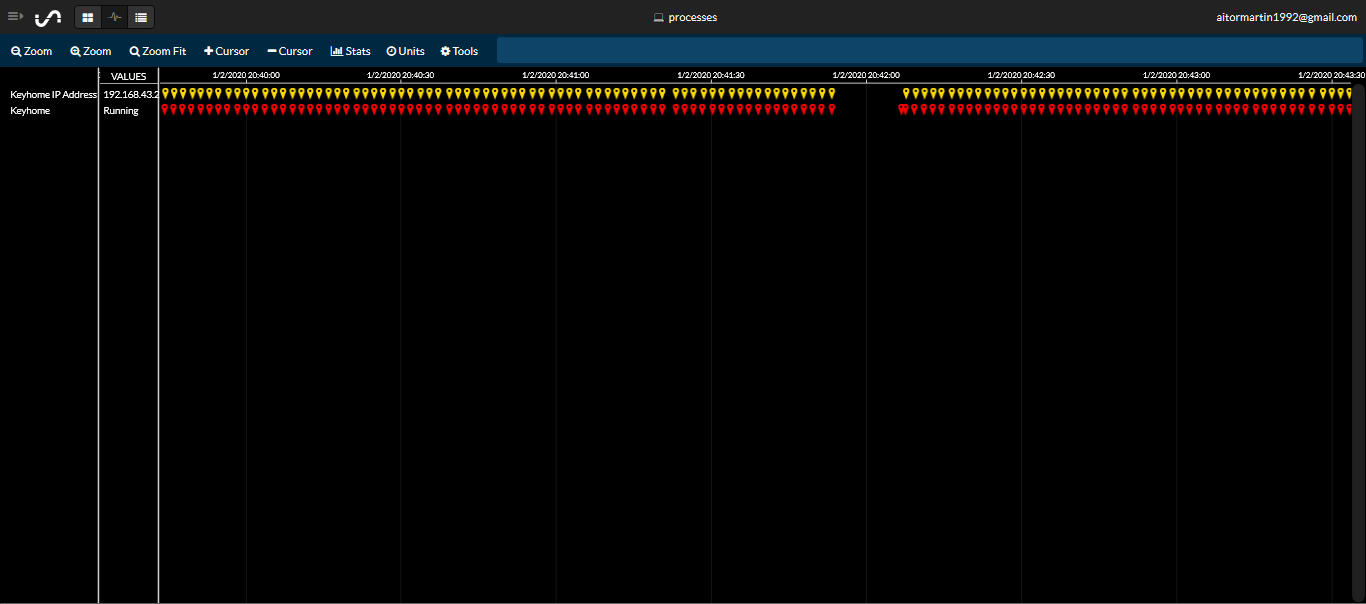
\includegraphics[scale=0.4]{fig/Monitorizacion.PNG}
\caption{Monitorización de la ejecución de un programa en la Raspberry Pi}
\label{fig:monitorizacion}
\end{figure}

En el caso de que se produzca una interrupción en el funcionamiento, el sistema de aviso alertará al propietario de la vivienda advirtiéndole de lo sucedido, tal como puede observarse en la figura~\ref{fig:aviso-ante-interrupcion-del-funcionamiento}. De esta manera, el anfitrión tendrá constancia de lo sucedido y podrá tomar las medidas que considere oportunas, como puede ser intercambiar la microSD de la Raspberry Pi para salvar posibles manipulaciones que pudieran haber ocurrido, o incluir por medio de su panel de control en Telegram las reservas que hubieran llegado en ese periodo de inactividad.

\begin{figure}[tbp]
\centering
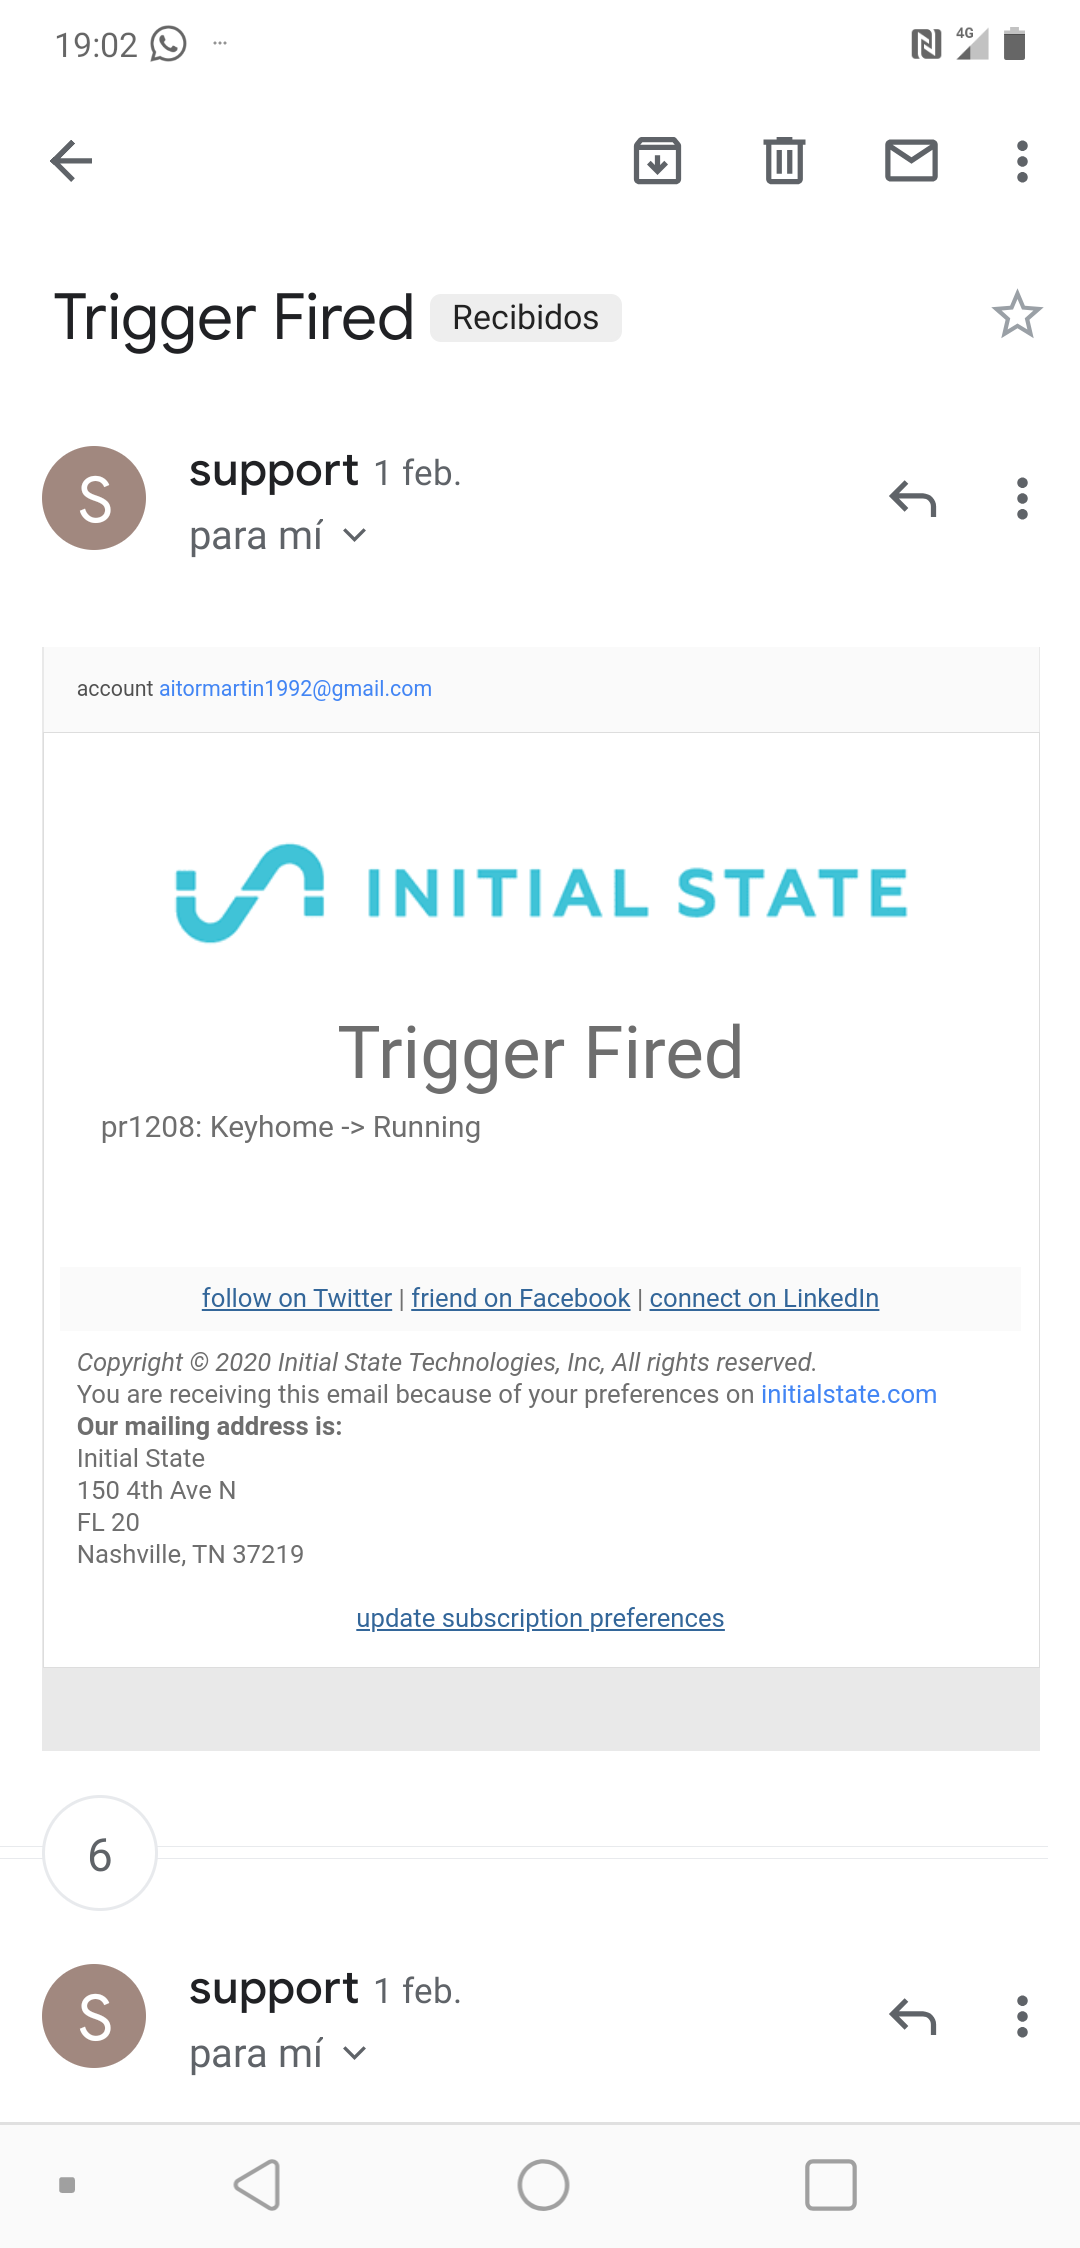
\includegraphics[scale=0.15]{fig/aviso-ante-interrupcion-del-funcionamiento.png}
\caption{Aviso ante una interrupción del funcionamiento}
\label{fig:aviso-ante-interrupcion-del-funcionamiento}
\end{figure}
